
% ---------------------------------------------
% Autor:        UOS, Arbeitsgruppe Software Engineering und CAU Kiel
%               mit Verbesserungen von Valentin Bruder (26.06.13)
% Beschreibung: Vorlage für Seminarausarbeitung
% Dateiname:    ausarbeitung.tex 
% Projekt:      Seminare
% erstellt am:  24.04.2013
% geändert am:  $Date$
% ---------------------------------------------

%%%%%%%%%%%%%%%%%%%%%%%%%%%%%%%%%%%%%%%%%%%%
%%%             Achtung!!                %%%
%%% In diesem Beispiel werden Pakete ver-%%%
%%% wendet, die ggf. nachinstalliert wer-%%%
%%% den müssen!                          %%%
%%%%%%%%%%%%%%%%%%%%%%%%%%%%%%%%%%%%%%%%%%%%


%%%%%%%%%%%%%%%%%%%%%%%%%%%%%%%%%%%%%%%%%%%%
%%% Es wird KOMA-Script verwendet        %%%
%%% welches in den meisten TeX-          %%%
%%% Distributionen enthalten ist!        %%%
%%%%%%%%%%%%%%%%%%%%%%%%%%%%%%%%%%%%%%%%%%%%
%\documentclass[a4paper, 11pt, DIV=11, listof=numbered, bibliography=numbered, pointlessnumbers]{scrartcl}
\documentclass[a4paper, 11pt, DIV=11, listof=numbered, numbers=noenddot]{scrartcl}

%%%%%%%%%%%%%%%%%%%%%%%%%%%%%%%%%%%%%%%%%%%%%%
%%%     benötigte Pakete                   %%%
%%%%%%%%%%%%%%%%%%%%%%%%%%%%%%%%%%%%%%%%%%%%%%
\usepackage[backend=biber,style=alphabetic,sortlocale=de]{biblatex}
\usepackage[utf8]{inputenc}     % Paket für Eingabekodierung (utf8 für die meisten aktuellen Linux-Distributionen): Umlaute
%\usepackage[latin1]{inputenc}  % Eingabekodierung für Windows falls UTF8 nicht unterstützt wird
\usepackage[ngerman]{babel}		% Deutsche Spracheigenheiten
\usepackage[autostyle=true,german=quotes]{csquotes}
\usepackage{amsmath}		% AMS Mathe und Symbolpakete für mehr Möglichkeiten
\usepackage{amsfonts}
%%\usepackage{amssymb}
% \usepackage{floatflt}
% \usepackage{float}
\usepackage{graphicx}		% Grafiken einbinden
\usepackage{xcolor}
\usepackage{hyperref}		% Erzeugt Verlinkungen im Dokument
\usepackage{url}			% erlaubt das einfache Schreiben von URLs
\usepackage{listings}		% für Listings (ftp://ftp.ctan.org/tex-archive/macros/latex/contrib/listings/listings.pdf)
\usepackage[T1]{fontenc} 	% Wichtig für Umlaute in PDFs
\usepackage{lmodern}		% Für bessere Schriftdarstellung trotz fontenc

%%%%%%%%%%%%%%%%%%%%%%%%%%%%%%%%%%%%%%%%%%%%%%
%%%      Weitere sinnvolle Pakete          %%%
%%%      ggf. Kommentar entfernen          %%%
%%%%%%%%%%%%%%%%%%%%%%%%%%%%%%%%%%%%%%%%%%%%%%

\usepackage{multirow}		% Zeilen in Tabellen zusammenfassen (http://tug.ctan.org/tex-archive/macros/latex/required/graphics/grfguide.pdf)
\usepackage{hhline}		% Horizontale Linien in Tabellen feiner gestalten

% Unterabbildungen können mit dem subfig-Paket realisiert werden.
% (z.B. Abb. 1a) (http://tug.ctan.org/tex-archive/macros/latex/contrib/subfig/subfig.pdf)
\usepackage{blindtext}

\usepackage{hyperref}
\usepackage{acronym}
\usepackage{subfigure}


% Sehr gute Möglichkeiten um Grafiken direkt in LaTeX zu erzeugen bietet Tikz (http://mirror.ctan.org/graphics/pgf/base/doc/generic/pgf/pgfmanual.pdf und http://www.statistiker-wg.de/pgf/tutorials.htm)
%\usepackage{tikz}		% 
%\usetikzlibrary[shapes.misc,shapes.geometric,arrows,decorations.pathmorphing,backgrounds,fit,positioning]

%Globale Einstellungen für das Listingspaket
\lstset{numbers=left,
	basicstyle=\ttfamily\small, 		% Setzt den Standardstil
	keywordstyle=\bfseries\small, 		% Setzt den Stil für Schlüsselwörter
	identifierstyle=\bfseries, 		% Identifier fett
	tabsize=2,				% Breite der Tabs
	showstringspaces=false,			% Leerzeichen in Strings nicht anzeigen
	commentstyle=\color{red!40}, 		% Stil für Kommentare
	stringstyle=\color{blue}, 		% Stil für Strings (gekennzeichnet mit "String")
	breaklines=true, 			% Zeilen werden umgebrochen
	numbers=left, 				% Zeilennummern links
	numberstyle=\tiny, 			% Stil für die Seitennummern
	frame=single, 				% Rahmen	
	backgroundcolor=\color{black!10}, 	% Hintergrundfarbe
	captionpos=b,				% Position der Listingunterschrift
	float
}

% define colors for code highlighting
\colorlet{punct}{red!60!black}
\definecolor{background}{HTML}{EEEEEE}
\definecolor{delim}{RGB}{20,105,176}
\definecolor{lightgray}{rgb}{0.95, 0.95, 0.95}
\definecolor{darkgray}{rgb}{0.4, 0.4, 0.4}
\definecolor{editorGray}{rgb}{0.95, 0.95, 0.95}
\definecolor{editorOcher}{rgb}{1, 0.5, 0} % #FF7F00 -> rgb(239, 169, 0)
\definecolor{editorGreen}{rgb}{0, 0.5, 0} % #007C00 -> rgb(0, 124, 0)
\definecolor{orange}{rgb}{1,0.45,0.13}		
\definecolor{olive}{rgb}{0.17,0.59,0.20}
\definecolor{brown}{rgb}{0.69,0.31,0.31}
\definecolor{purple}{rgb}{0.38,0.18,0.81}
\definecolor{lightblue}{rgb}{0.1,0.57,0.7}
\definecolor{lightred}{rgb}{1,0.4,0.5}
\colorlet{numb}{magenta!60!black}
\newcommand\YAMLcolonstyle{\color{red}\mdseries}
\newcommand\YAMLkeystyle{\color{black}\bfseries}
\newcommand\YAMLvaluestyle{\color{blue}\mdseries}

\lstdefinelanguage{json}{
	basicstyle=\footnotesize\selectfont\ttfamily,
	showstringspaces=false,
	breaklines=true,
	frame=lines,
	backgroundcolor=\color{white},
	literate=
	*{:}{{{\color{punct}{:}}}}{1}
	{,}{{{\color{punct}{,}}}}{1}
	{\{}{{{\color{delim}{\{}}}}{1}
	{\}}{{{\color{delim}{\}}}}}{1}
	{[}{{{\color{delim}{[}}}}{1}
	{]}{{{\color{delim}{]}}}}{1},
}

\lstdefinelanguage{yaml}{
	keywords={true,false,null,y,n},
	keywordstyle=\color{darkgray}\bfseries,
	basicstyle=\footnotesize\selectfont\ttfamily,    
	showstringspaces=false,
	breaklines=true,
	frame=lines,
	sensitive=false,
	comment=[l]{\#},
	morecomment=[s]{/*}{*/},
	commentstyle=\color{purple}\ttfamily,
	moredelim=[l][\color{orange}]{\&},
	moredelim=[l][\color{magenta}]{*},
	moredelim=**[il][\YAMLcolonstyle{:}\YAMLvaluestyle]{:},   % switch to value style at :
	morestring=[b]',
	morestring=[b]",
	literate =    {---}{{\ProcessThreeDashes}}3
	{>}{{\textcolor{red}\textgreater}}1     
	{|}{{\textcolor{red}\textbar}}1 
	{\ -\ }{{\mdseries\ -\ }}3,
}


%%%%%%%%%%%%%%%%%%%%%%%%%%%%%%%%%%%%%%%%%%%%%%%%%%%%%%%%%
%%% Ein paar Hilfskommandos, die nützlich sein können %%%
%%%%%%%%%%%%%%%%%%%%%%%%%%%%%%%%%%%%%%%%%%%%%%%%%%%%%%%%%
\newcommand{\code}[1]{\textsf{#1}}	% Code in Text
\newcommand{\pkg}[1]{\textsf{#1}}	% Paketnamen
\newcommand{\class}[1]{\textsf{#1}} 	% Klassennamen
\newcommand{\idx}[1]{_\text{#1}} 	% schreibt in Formeln einen nicht kursiven Index

% Einbindung der Biblatex-Datei
\addbibresource{literatur.bib}


%%%%%%%%%%%%%%%%%%%%%%%%%%%%%%%%%%%%%%
%%% Einstellungen für das Dokument %%%
%%%%%%%%%%%%%%%%%%%%%%%%%%%%%%%%%%%%%%

% Der Titel wird hier eingetragen
\title{\enquote{Trash Bash} - Das mobile Müllmeldesystem}

% Der/die Verfasser wird hier angegeben
\author{Kevin Rüter, Wilko Müller}


%%%%%%%%%%%%%%%%%%%%%%%%%%%%%%%%%%%%%%%%%%%%%
%%% Hier beginnt das eigentliche Dokument %%%
%%%%%%%%%%%%%%%%%%%%%%%%%%%%%%%%%%%%%%%%%%%%%

\begin{document}
	
	
	%%%%%%%%%%%%%%%%%%
	%%% Titelblatt %%%
	%%%%%%%%%%%%%%%%%%
	\begin{titlepage}
		\begin{center}
			\vspace*{1.5cm}
			\begin{Large}
				\textbf{Universit\"at Osnabr\"uck}
			\end{Large}
			
			\noindent\hrulefill
			\\[3.5cm]
			BERICHT \\[1cm]
			zum Seminar \\[1cm]
			\textbf{Standortbasierte Dienste} \\[1.5cm]    % Seminartitel eintragen 
			im Wintersemester 2019/2020 \\[1.5cm]   % Semester / Datum eintragen
			Thema: \\[0.5cm]
			\textbf{\enquote{Trash Bash} - Das mobile Müllmeldesystem} \\[2cm]        % Titel des eigenen Seminarthemas eintragen
			Erstellt am \today
		\end{center}
		\vfill
		\begin{flushleft}
			Vorgelegt von: 
			\hfill \parbox{60mm}{Kevin Rüter} \\  % Eigene Daten einsetzen
			\hfill \parbox{60mm}{Wilko Müller}
		\end{flushleft}
	\end{titlepage}
	%%% end title page
	
	
	%%%%%%%%%%%%%%%%%%%%%%%%%%%%%%%%%%%%%%%%%%%%%%%%%%%%%
	%%% Inhaltsverzeichnis mit römischen Seitenzahlen %%%
	%%%%%%%%%%%%%%%%%%%%%%%%%%%%%%%%%%%%%%%%%%%%%%%%%%%%%
	\newpage
	\pagenumbering{roman}
	\tableofcontents 
	
	
	%%%%%%%%%%%%%%%%%%%%%%%%%%%%%%%%%%%%%%%%%%%%%%%%%%%%%%%%%%%%%%%
	%%% Start des Dokumenteninhalts mit arabischen Seitenzahlen %%%
	%%%%%%%%%%%%%%%%%%%%%%%%%%%%%%%%%%%%%%%%%%%%%%%%%%%%%%%%%%%%%%%
	
	\newpage
	\pagenumbering{arabic}
	
	\maketitle
	
	\begin{abstract}
		\noindent Im Folgenden wird die Funktionsweise der App „Trash Bash“ beschrieben. 
			Sie ist im Rahmen der Veranstaltung „Standortbasierte Dienste“ im Wintersemester 2019/2020 an der Universität Osnabrück entstanden.
	\end{abstract}

	\section{Einleitung}
	...

	\section{Grundlagen}
	In diesem Abschnitt werden zunächst die grundlegenden Technologien aufgeführt, die innerhalb des entwickelten Systems zum Einsatz kommen.

	\subsection{Datenbank}
	Im Rahmen der Veranstaltung wurde für die Abschlussaufgabe eine Datenbank-Tabelle bereitgestellt.
	Diese wurde auf einer Instanz des Datenbanksystems \textit{PostgreSQL} erstellt \cite{@Postgresql}.
	Dieses ist ein freies, objektrelationales Datenbanksystem, welches die Datenbanksprache \textit{SQL} unterstützt.\\
	Das Schema der Tabelle \enquote{trash}, welche bereitgestellt wurde, ist in Tabelle \ref{table:db} zu sehen.

	\begin{table}[h]
		\begin{center}
	
		\begin{tabular}{|l|l|c|}
			\hline
			\textbf{Spalte} & \textbf{Typ} & \textbf{NULL?} \\ \hline
			$id$              & serial        & -                 					\\ \hline
			$time$            & timestamp     & -                 					\\ \hline
			$username$        & varchar       & -                 					\\ \hline
			$latitude$        & real          & -                 					\\ \hline
			$longitude$       & real          & -                 					\\ \hline
			$hausmuell$       & boolean       & -                 					\\ \hline
			$gruenabfall$     & boolean       & -                 					\\ \hline
			$sperrmuell$      & boolean       & -                 					\\ \hline
			$sondermuell$     & boolean       & -                 					\\ \hline
			$photo$           & varchar       & \checkmark                 	\\ \hline
		\end{tabular}
	\caption{Schema der Datenbank-Tabelle \enquote{trash}}
	\label{table:db} 
		\end{center}
	\end{table}
	
	\subsection{REST}\label{ssec:rest}
	Der REST-Architekturstil ist eine Abstraktion verschiedener Elemente, wie die Verarbeitung, Verbindung und Repräsentation von Daten \cite{WebArch}. Die Kommunikation über REST ist mit dem \textit{Hypertext Transfer Protocol} (HTTP) realisiert, wobei sogenannte Ressourcen üblicherweise mit einer entsprechenden HTTP-Methode, wie GET, POST, PUT oder DELETE angefordert werden. Diese Methoden werden auch \enquote{CRUD-Operationen}\footnote{Create, Read, Update und Delete} genannt und entsprechen oftmals dem jeweiligen Anforderungstyp \cite{@CRUD}. So wird üblicherweise die Methode GET verwendet, um Daten von einer Ressource anzufordern, während die Methoden POST oder PUT angeben, Daten innerhalb der Ressource hinzuzufügen oder zu aktualisieren. DELETE suggeriert einen Löschvorgang.\\
	Die Darstellung und Anforderung einer Ressource wird über \textit{Uniform Resource Identifiers (URIs)} \cite{RFC3986} verrichtet. Ein Beispiel für eine Anfrage verschiedener Ressourcen wird in Abbildung \ref{fig:rest} gezeigt, bei der ein Nutzer inklusive seiner \enquote{Posts} und \enquote{Follower} anhand der ID als Übergabeparameter ausgelesen werden soll. Ersichtlich ist, dass für die Nutzerinformation, die Posts, sowie Follower des Nutzers separate Anfragen an den Server gesendet werden, um diese Daten zusammenzuführen.
	\begin{figure}[!htbp]
		\centering
		
\includegraphics[width=0.99\textwidth]{img/rest.png}
		\caption{Kommunikation mit REST (\textit{Quelle:} \url{https://www.howtographql.com/basics/1-graphql-is-the-better-rest/} [Stand: 16.05.2020])}\label{fig:rest}
	\end{figure}

	\subsection{Frameworks}
	Im Folgenden werden die Frameworks aufgelistet, die im Rahmen dieses Projektes genutzt wurden.

	\subsubsection{Apache Cordova}\label{sssec:cordova}
	Das Framework \textit{Apache Cordova}, welches früher unter dem Namen \textit{PhoneGap} bekannt war, ist ein Tool zum Erstellen mobiler, clientseitiger Anwendungen \cite{@Cordova}.
	Mit diesem ist es beispielweise möglich, hybride Anwendungen sowohl für das Betriebssystem \textit{iOS} von \textit{Apple}, so wie auch für \textit{Android} der Firma \textit{Google}, zu entwickeln.
	Hybrid bedeutet in diesem Kontext, dass eine Applikation mit gängigen Web-Standards, wie \textit{HTML}, \textit{CSS} und \textit{Javascript}, entwickelt und die erstellte Anwendung dann für mehrere Systeme mit derselben \enquote{Codebasis} erstellt werden kann.

	\subsubsection{Ionic}\label{sssec:ionic}
	Das \textit{Ionic Framework} ist ein freies, clientseitiges Web-Framework zur Erstellung mobiler Anwendungen \cite{@Ionic}.
	Im \enquote{Build-Prozess} einer Anwendung setzt dieses auf das in Abschnitt \ref{sssec:cordova} genannte \textit{Apache Cordova}.\\
	Ionic soll den Entwicklungsprozess mobiler Anwendungen erleichtern, indem bereits vorgefertige UI-Komponenten oder Plugins bereitgestellt werden, die vom Entwickler lediglich eingebunden werden müssen.
	Um dies zu bewerkstelligen, setzt das Framework auf die Grundstruktur eines anderen Frameworks: \textit{Angular} \cite{@Angular}.

	\subsubsection{Express}\label{sssec:express}
	Um eine Serverstruktur zu entwickeln, welche eine Kommunikation über den in Abschnitt \ref{ssec:rest} genannten Architekturstil \textit{REST} ermöglicht, wird das Framework \textit{Express.js} verwendet \cite{@Express}.
	Dieses ist ein serverseitiges Web-Framework, welches auf der ebenso serverseitigen Plattform \textit{Node.js} basiert \cite{@Nodejs}.
	
	\section{Komponenten}
	Im Folgenden werden die Komponenten beschrieben, welche zur Erstellung der App \enquote{Trash Bash} genutzt wurden:

	\begin {itemize}
	\item \textbf{Frontend / App}
		\begin {itemize}
		\item \textbf{Angular:} Dient als Hauptkomponente zur Strukturierung der App. Vereinfacht beispielsweise den Umgang mit Webinhalten durch Services.
		\item \textbf{Ionic:} Fügt einige UI-Komponenten zu Angular hinzu, die sich durch gutes Design in Android und iOS Apps auszeichnen.
		\item \textbf{Leaflet:} Die Müllmeldekarte wird durch Leaflet eingestellt. Mit Leaflet lassen sich Karten in Webseiten und Apps einbinden und zudem mit Markern und Popups erweitern.
		\item \textbf{Cordova:} Wird für den Build-Prozess der App verwendet.
		\end {itemize}
	\item \textbf{Backend / Server}
		\begin {itemize}
			\item \textbf{Express.js:} Stellt die benötigten HTTP-Server Funktionen bereit, für die Schnittstelle zwischen App und Datenbank. Zudem wird, um die Bilder hochzuladen, die \textit{fileupload}-Funktion genutzt.
			\item \textbf{Crypto:} Node-Paket, welches benötigt wird, um den \textit{md5}-Hashwert für den Dateinamen der Bilder zu berechnen.
			\item \textbf{PostgreSQL:} Stellt die Verbindung vom Server-Skript zur Datenbank her.
			\item \textbf{GeoJSON:} Wird verwendet, um die Einträge aus der Datenbank, welche über HTTP GET angefordert werden, im GeoJSON-Format \cite{@Geojson} zurückzusenden. 
		\end {itemize}
	\end {itemize}

	Im weiteren Verlauf des Abschnittes werden diese Komponenten genauer beschrieben.

	\subsection{Frontend / App}
	\subsubsection{Pages}
	Im Folgenden werden die \enquote{Page}-Komponenten der entwickelten Ionic-App beschrieben, welche von beispielhaften Screenshots begleitet werden, um die Funktionalitäten zu visualisieren.
	
	\paragraph{Map}
	\textbf{}\\
	\textbf{}\\
	Die Page-Komponente \enquote{Map} stellt den Hauptteil der Anwendung dar.
	Hier wird über den gesamten Bildschirm eine Karte über das Framework \textit{Leaflet} dargestellt \cite{@Leaflet}.
	Dies ist in Abbildung \ref{fig:app-map} zu sehen.
	\begin{figure}[!htbp]
		\centering
		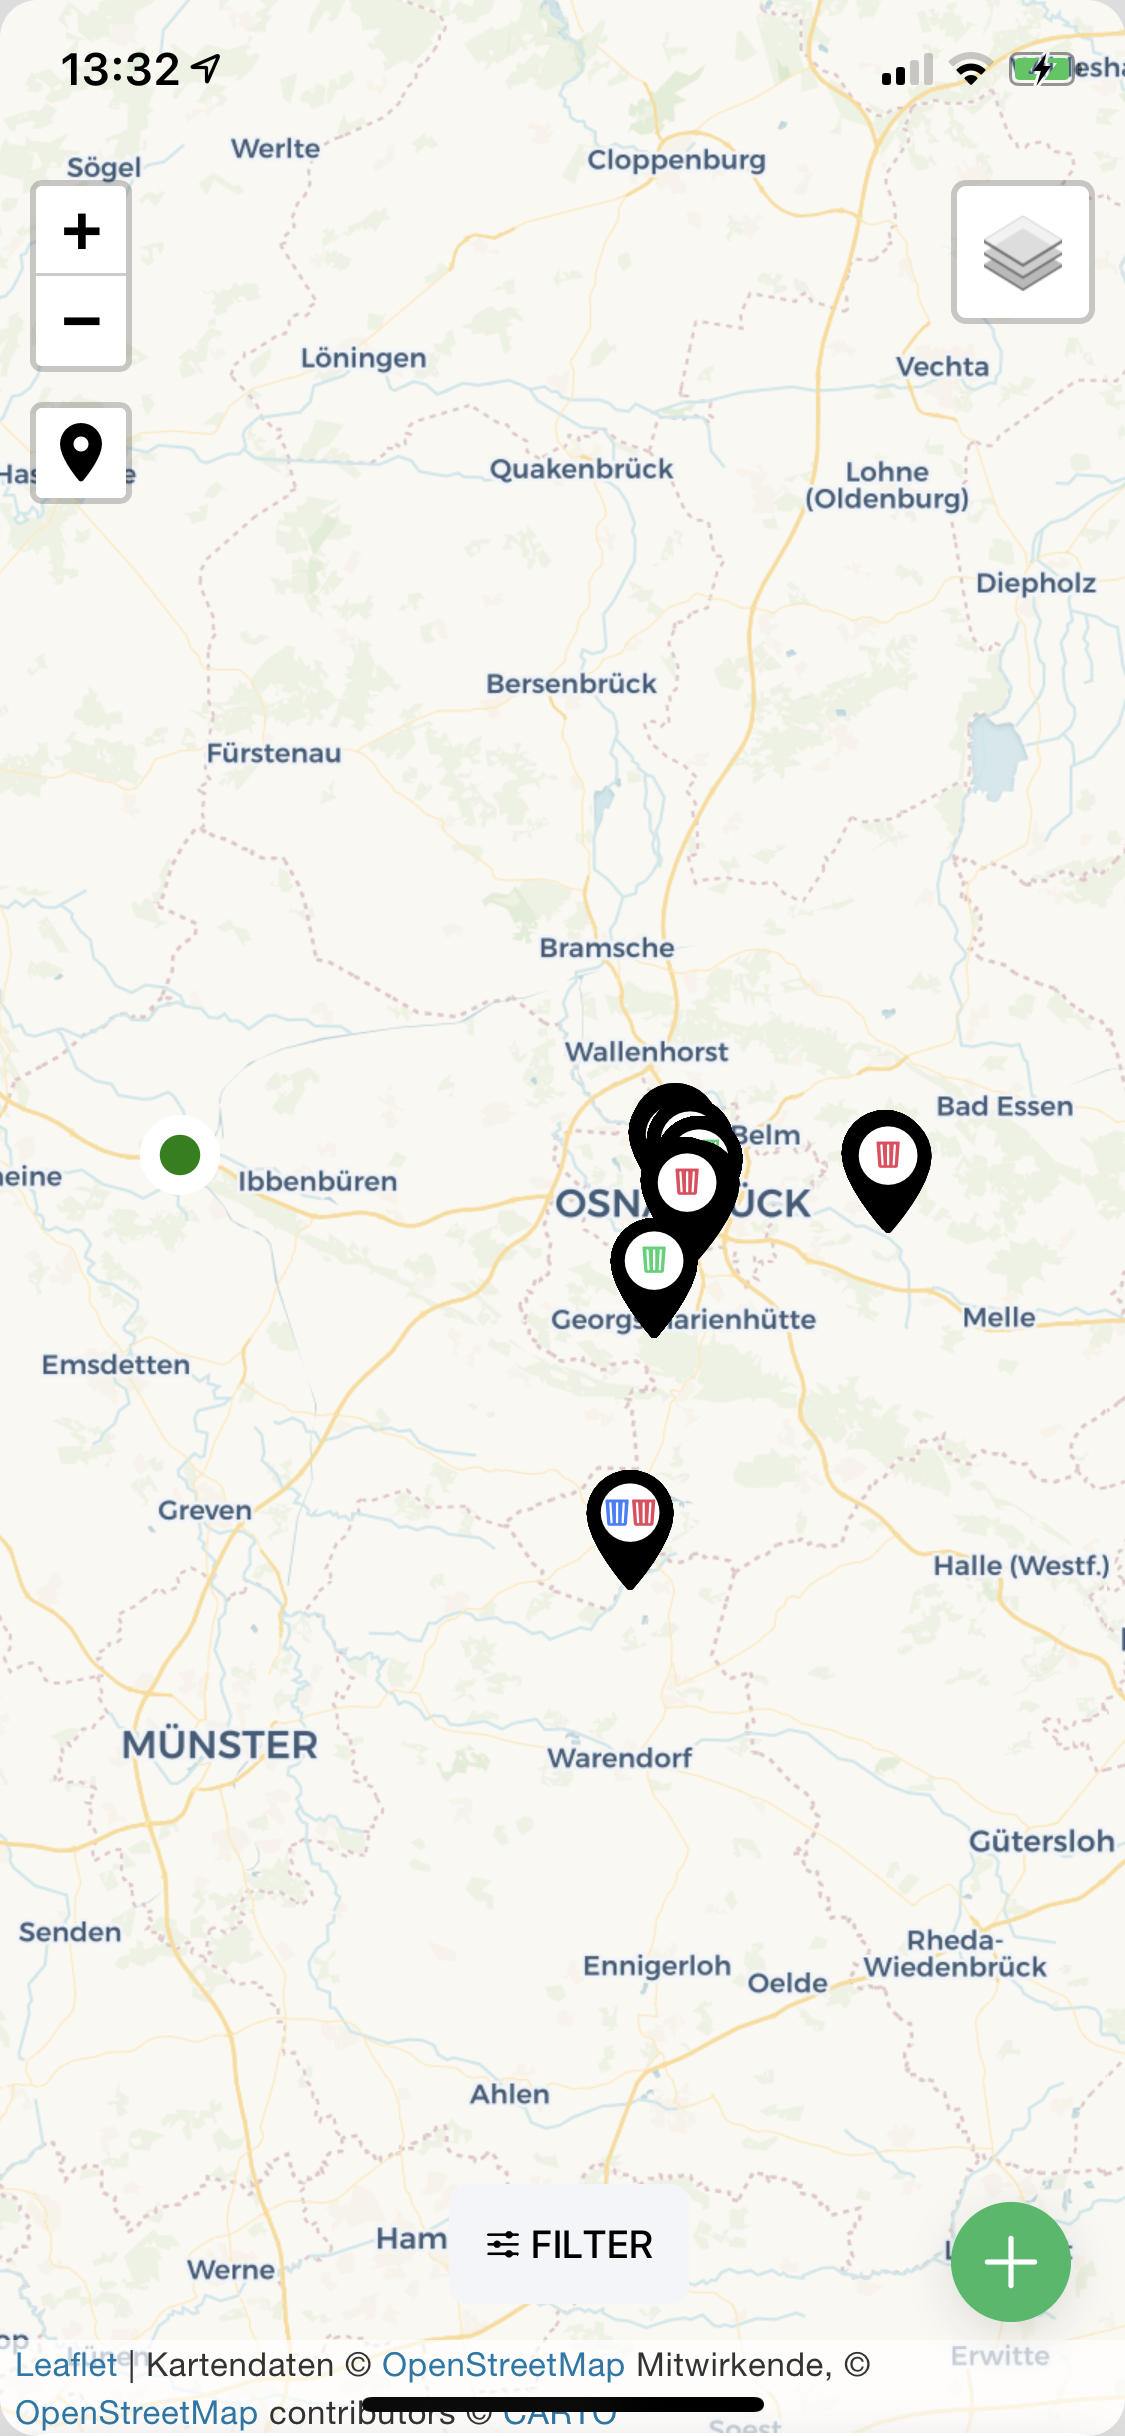
\includegraphics[width=0.25\textwidth]{img/app/map.png}
		\caption{Map-Page}\label{fig:app-map}
	\end{figure}
	Hier ist ein grün-weißer, in der App animierter, Kreis zu sehen, der den aktuellen Nutzerstandort visualisiert. Hier ist es möglich, den Nutzerstandort zu verfolgen (siehe Abbildung x).
	\begin{figure}[!htbp]
		\centering
		\subfigure[Nutzer wird nicht verfolgt]{\centering
\includegraphics[width=0.1\textwidth]{img/app/location-off.png}}\hfill%
		\subfigure[Nutzer wird verfolgt]{\centering
\includegraphics[width=0.1\textwidth]{img/app/location-on.png}}\hfill%
		\caption{Trigger zur \enquote{Verfolgung} der Position des Nutzers auf der Karte}\label{fig:app-map-track-user}
	\end{figure}
	Zudem sind verschiedene Marker zu sehen. Diese sind gemeldete Müllablagerungen von Nutzern. Die Mülltypen des \enquote{Reports}, wie \textit{Hausmüll}, \textit{Grünabfall}, \textit{Sperrmüll} oder \textit{Sondermüll}, sind innerhalb des Markers illustriert. 
	Klickt man nun auf einen dieser Marker, werden weitere Informationen zum gewählten Report angezeigt (siehe Abbildung \ref{fig:app-map-report}).
	\begin{figure}[!htbp]
		\centering
		\subfigure[Mit gemeldetem Bild]{\centering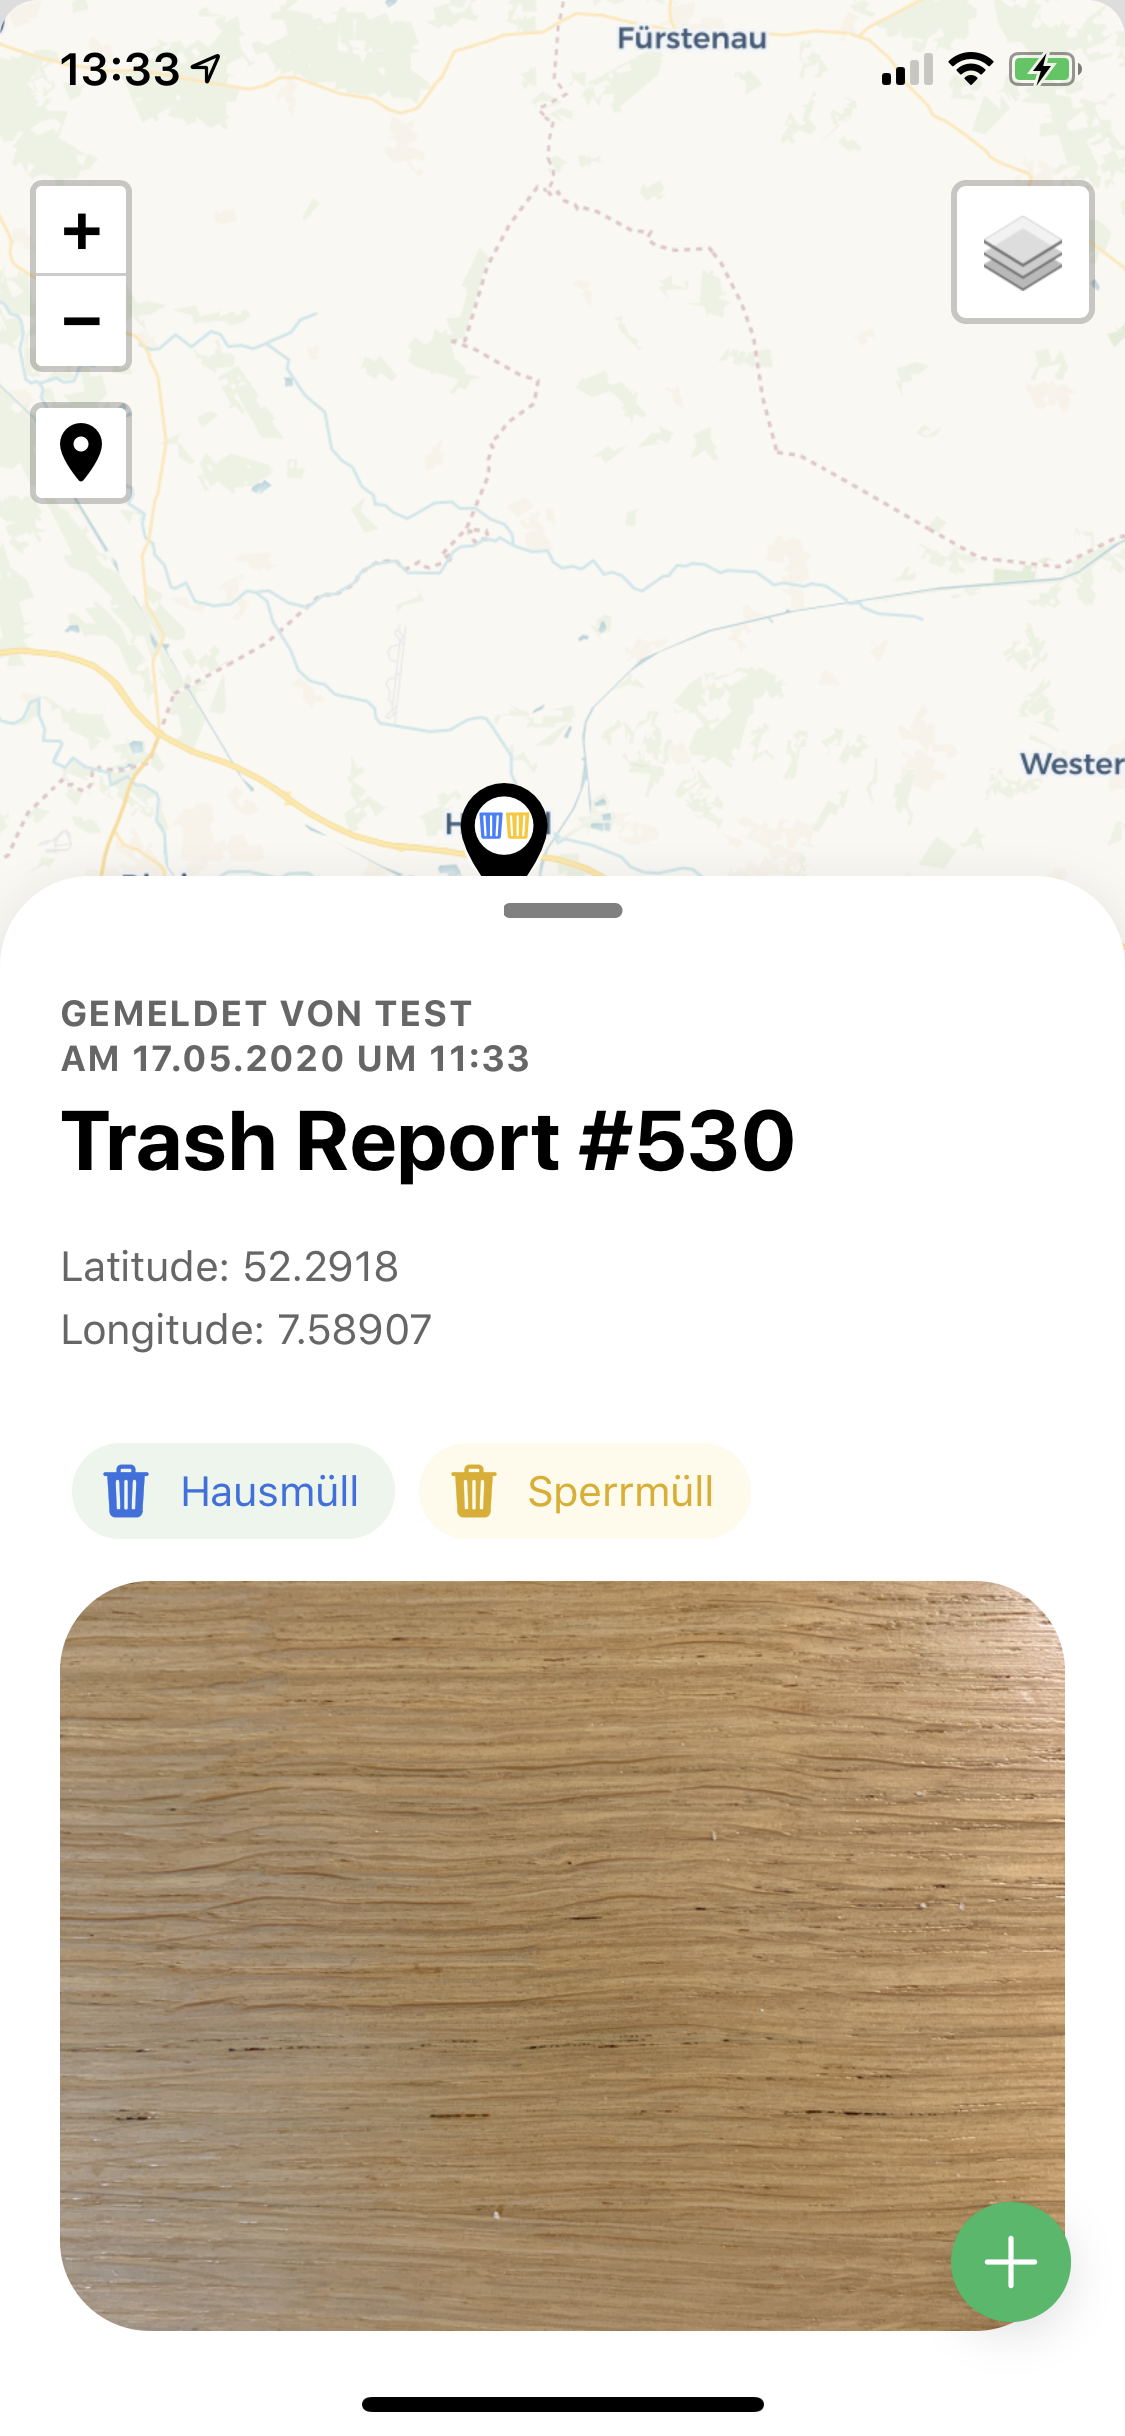
\includegraphics[width=0.3\textwidth]{img/app/map-report.png}}\hfill%
		\subfigure[Ohne gemeldetem Bild]{\centering\includegraphics[width=0.3\textwidth]{img/app/map-report-no-image.png}}\hfill%
		\caption{Map-Page - Report Infos}\label{fig:app-map-report}
	\end{figure}
	In diesem ist auch eine Legende zu sehen, welche die einzelnen Farben zu den Mülltypen erläutert (siehe Abbildung \ref{fig:legend}).
	\begin{figure}[!htbp]
		\centering
		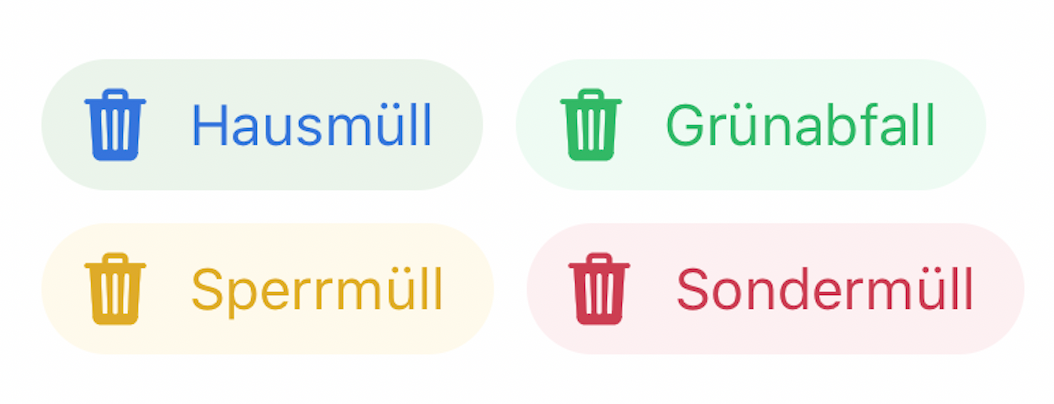
\includegraphics[width=0.25\textwidth]{img/app/legend.png}
		\caption{Map-Page - Legende zu den einzelnen Typen der Müllablagerung}\label{fig:legend}
	\end{figure}
	Um die weiteren Informationen wieder zu schließen, kann hier für eine \enquote{Swipe}-Geste verwendet werden. Um dies zu ermöglichen, wurde das Ionic-Plugin \enquote{Gesture Controller} von Ionic verwendet.\\
	Wie die Map-Komponente initialisiert wird, ist folgend beschrieben:
	\begin {itemize}
		\item Die Initialisierung der Leaflet Karte wird von der initializeMap-Methode der Angular Map Page durchgeführt. Als Kartendatenprovider kann zwischen \href{https://www.openstreetmap.org}{Open Street Maps} und \href{http://voyager.basemaps.cartocdn.com}	{Voyager} entschieden werden. Die Auswahl kann über die \textit{leaflet-control-layers-expanded} Schaltfläche in der oberen, rechten Ecke getroffen werden.
		\item Ebenfalls wird in der \textit{initializeMap}-Methode der Standort des App-Nutzers ermittelt. Dazu benutzen wir die Klasse Geolocation aus dem Ionic Native Framework. Zunächst wird die momentane Position in Form von Längen- und Breitengrad durch 					\textit{getCurrentPosition} abgerufen. Da diese Methode asynchron abläuft, muss die komplette \textit{initializeMap}-Methode als \textit{async} definiert werden und mit dem \textit{await} Statement vor dem Aufruf auf die Erfüllung der zurückgegebenen 				\textit{Promise} gewartet werden. Die erhaltenen Daten werden daraufhin einem Standortmarker übergeben.
			Damit die Position des Users stets aktuell bleibt, setzen wir den \textit{UserLocationObserver} aus Ionic Native ein und lassen den Standortmarker auf etwaige Standortveränderungen horchen. So wird der Marker bei einem Standortwechsel verschoben.
		\item Die gemeldeten illegalen Müllablagerungen werden mit einem Leaflet Marker an den jeweiligen Koordinaten dargestellt. Im Abschnitt \hyperref[sec:Filter] {Filter} wird genauer auf das Abrufen der Daten eingegangen.

	\end {itemize}

	\paragraph{Report}
	\textbf{}\\
	\textbf{}\\
	Um eine Meldung von Müllablagerungen zu realisieren, wurde eine weitere Page-Komponente entwickelt, welches durch ein sogenanntes \enquote{Modal} abgebildet wird.
	Die Funktionsweise wird folgend erläutert:
	\begin {itemize}
		\item Die Meldung einer illegalen Müllablagerung wird über den grünen Knopf mit dem Plus in der unteren rechten Ecke der Map-Page gestartet. Daraufhin öffnet sich ein \textit{Angular Modal} Dialog-Fenster, in welchem die Daten zur Müllablagerung vom Nutzer eingetragen 					werden können. Es wird ein \textit{Modal} benutzt, da man es über die Leaflet-Karte legen kann und somit diese im Hintergrund, bei der Eingabe der Mülldetails, visualisiert bleibt. Zudem sorgt die \textit{Ionic}-Funktion \textit{backdrop} für den grauen 					Schleier über der Karte im Hintergrund.
		\item Die Eingabe des Nutzernamens wird über ein \textit{Ionic input} realisiert. Dieser wird in der HTML-Template-Datei zum Müllmelde-Modal \textit{„add.page.html“} definiert. In demselben Template wird auch eine \textit{Ionic-list} angelegt, bestehend aus jeweils 				einem \textit{label} und einer \textit{checkbox}. Die Liste wird mit den vier verschiedenen Kategorien von Müllablagerungen bestückt. Im \textit{label} wird der Name angezeigt und die \textit{checkbox} markiert ob der jeweilige Müll-Typ vorhanden ist.
			Damit auch Bilder der Müllablagerung mitgesendet werden können benötigen wir aus\textit{ Ionic Native} die \textit{Camera}-Klasse. Diese beruht auf dem \textit{Cordova-Camera-Plugin} um an die Hardware Funktionen der Smartphone-Kamera und die 				gespeicherten Fotos zu gelangen. Da das Hinzufügen von Bildern optional ist, wird vor dem Absenden der Meldung dem Nutzer ein \textit{Ionic action-sheet} präsentiert. Dieses \textit{Ionic} Gestaltungselement ist dazu gedacht eine Auswahl von Optionen zu 				präsentieren. Es gibt zwei \textit{action-sheets} im Müllmeldeprozess. Im ersten kann ausgewählt werden, ob ein Bild angefügt werden soll. Beantwortet man dies mit „Nein“ wird die Meldung direkt an die Datenbank gesendet. Wird „Ja“ gewählt kommt ein 				zweites \textit{action-sheet} in welchem man sich entscheiden kann, ob man ein neues Bild mit der Kamera aufnehmen möchte oder eins aus der Fotogalerie hochladen möchte. Die beiden Funktionen werden plattformunabhängig von \textit{Cordova} über 				\textit{Ionic} bereitgestellt. Die von uns erstellte Funktion \textit{getImage(sourceType: number)} speichert das Bild aus der jeweiligen Quelle im JPEG-Format ab und löst \textit{sendReport} aus. Die Meldung ist dann abgeschlossen und man gelangt wieder zurück auf die Karte. Hier wird dann zusätzlich der soeben erstellte Report auf der Karte angezeigt.
	\end{itemize}
	Zur weiteren Visualisierung sind Screenshots zur Meldung einer Müllablagerung in Abbildung \ref{fig:app-report} zu sehen.
	\begin{figure}[!htbp]
		\centering
		\subfigure[Initial]{\centering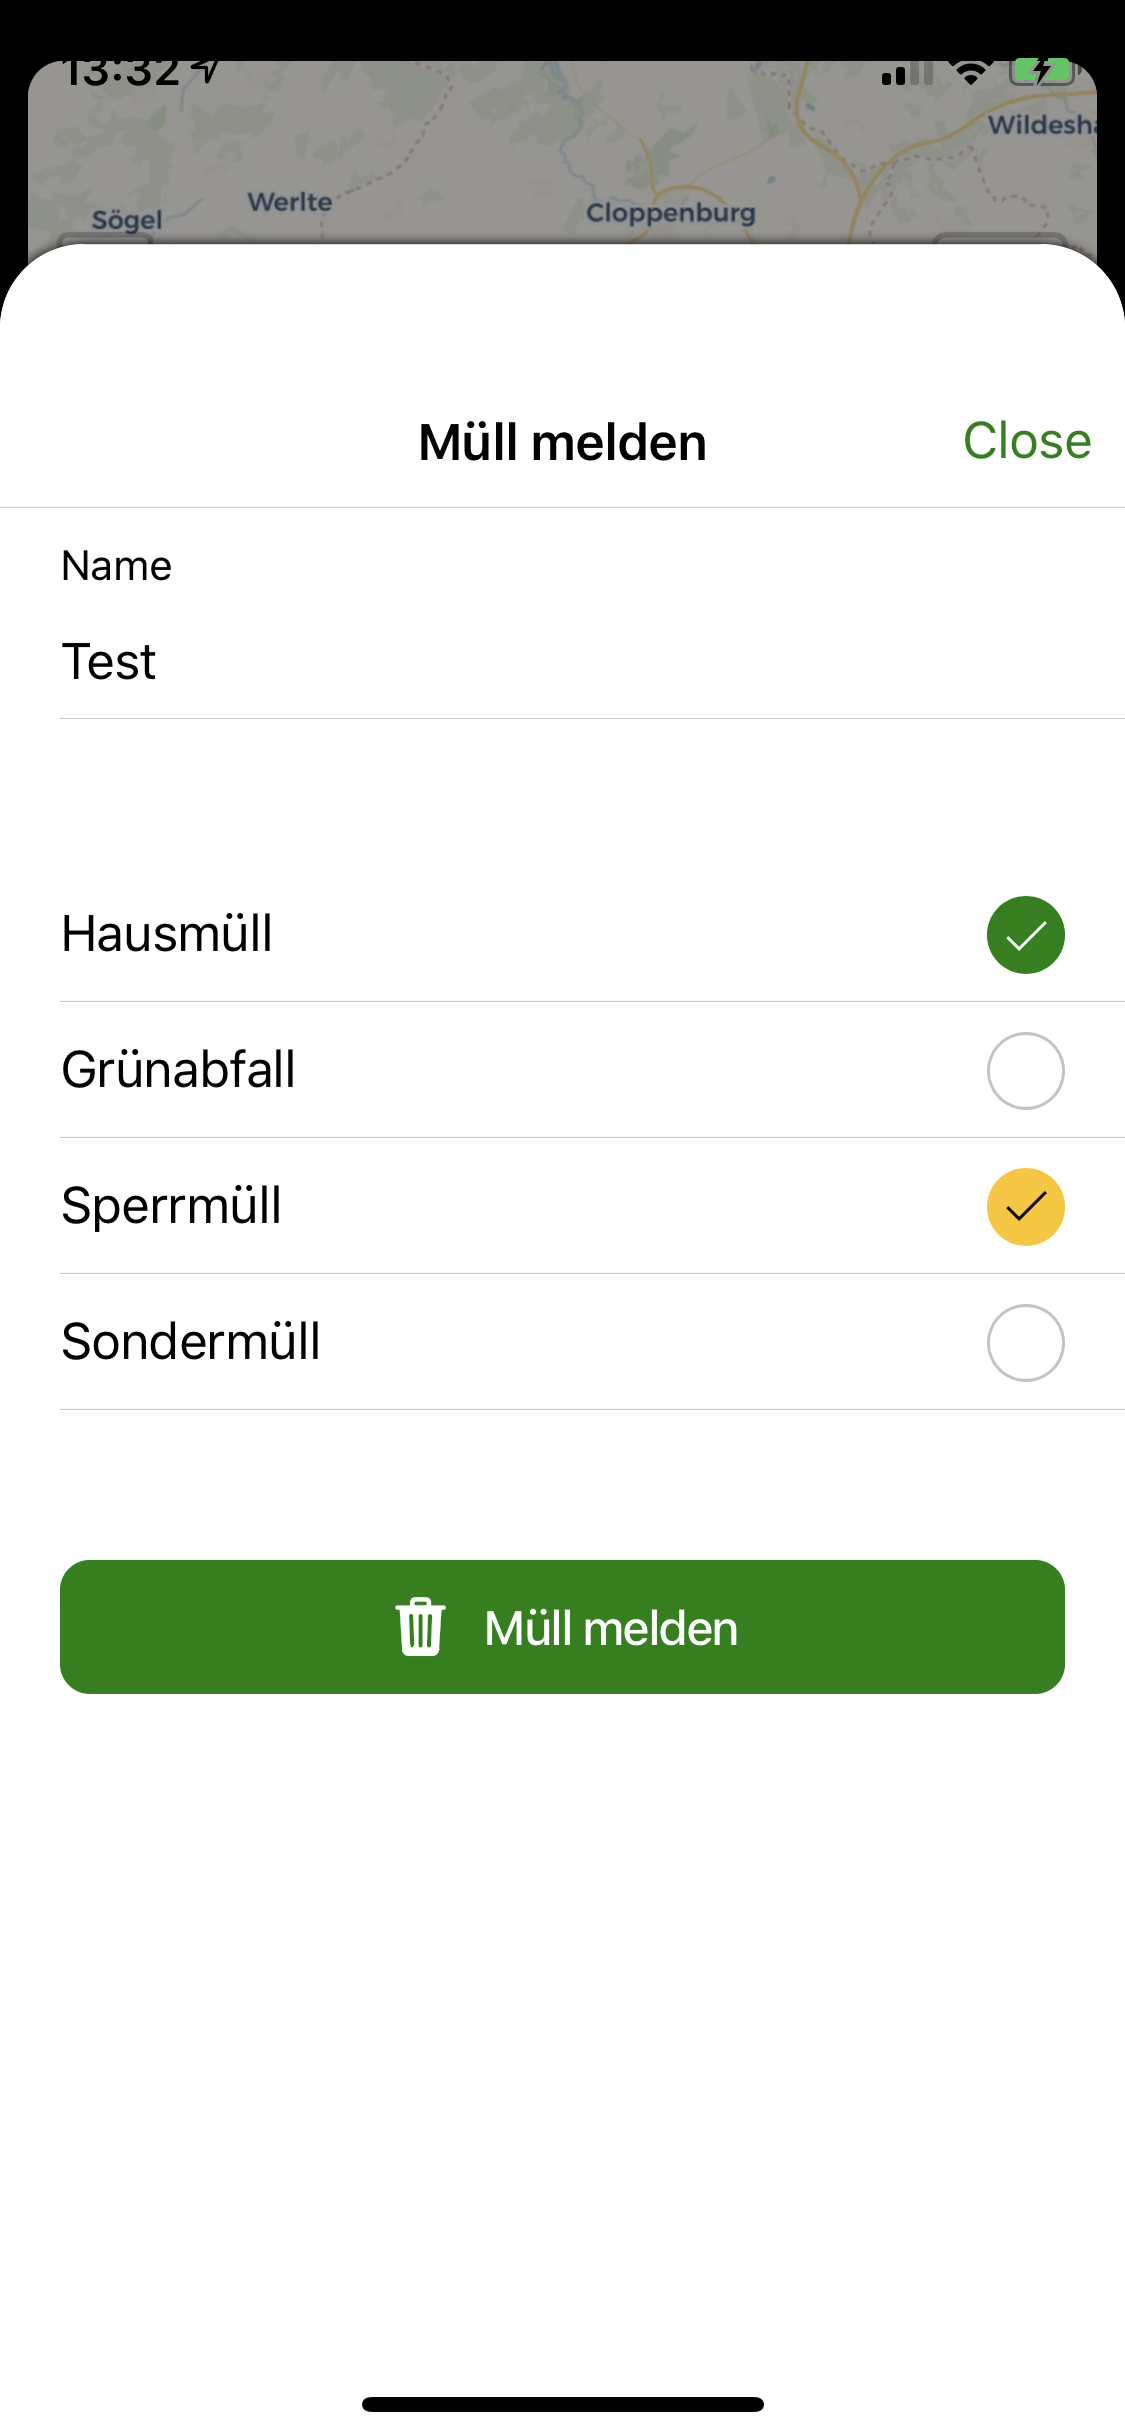
\includegraphics[width=0.2\textwidth]{img/app/report.png}}\hfill%
		\subfigure[Foto hinzufügen]{\centering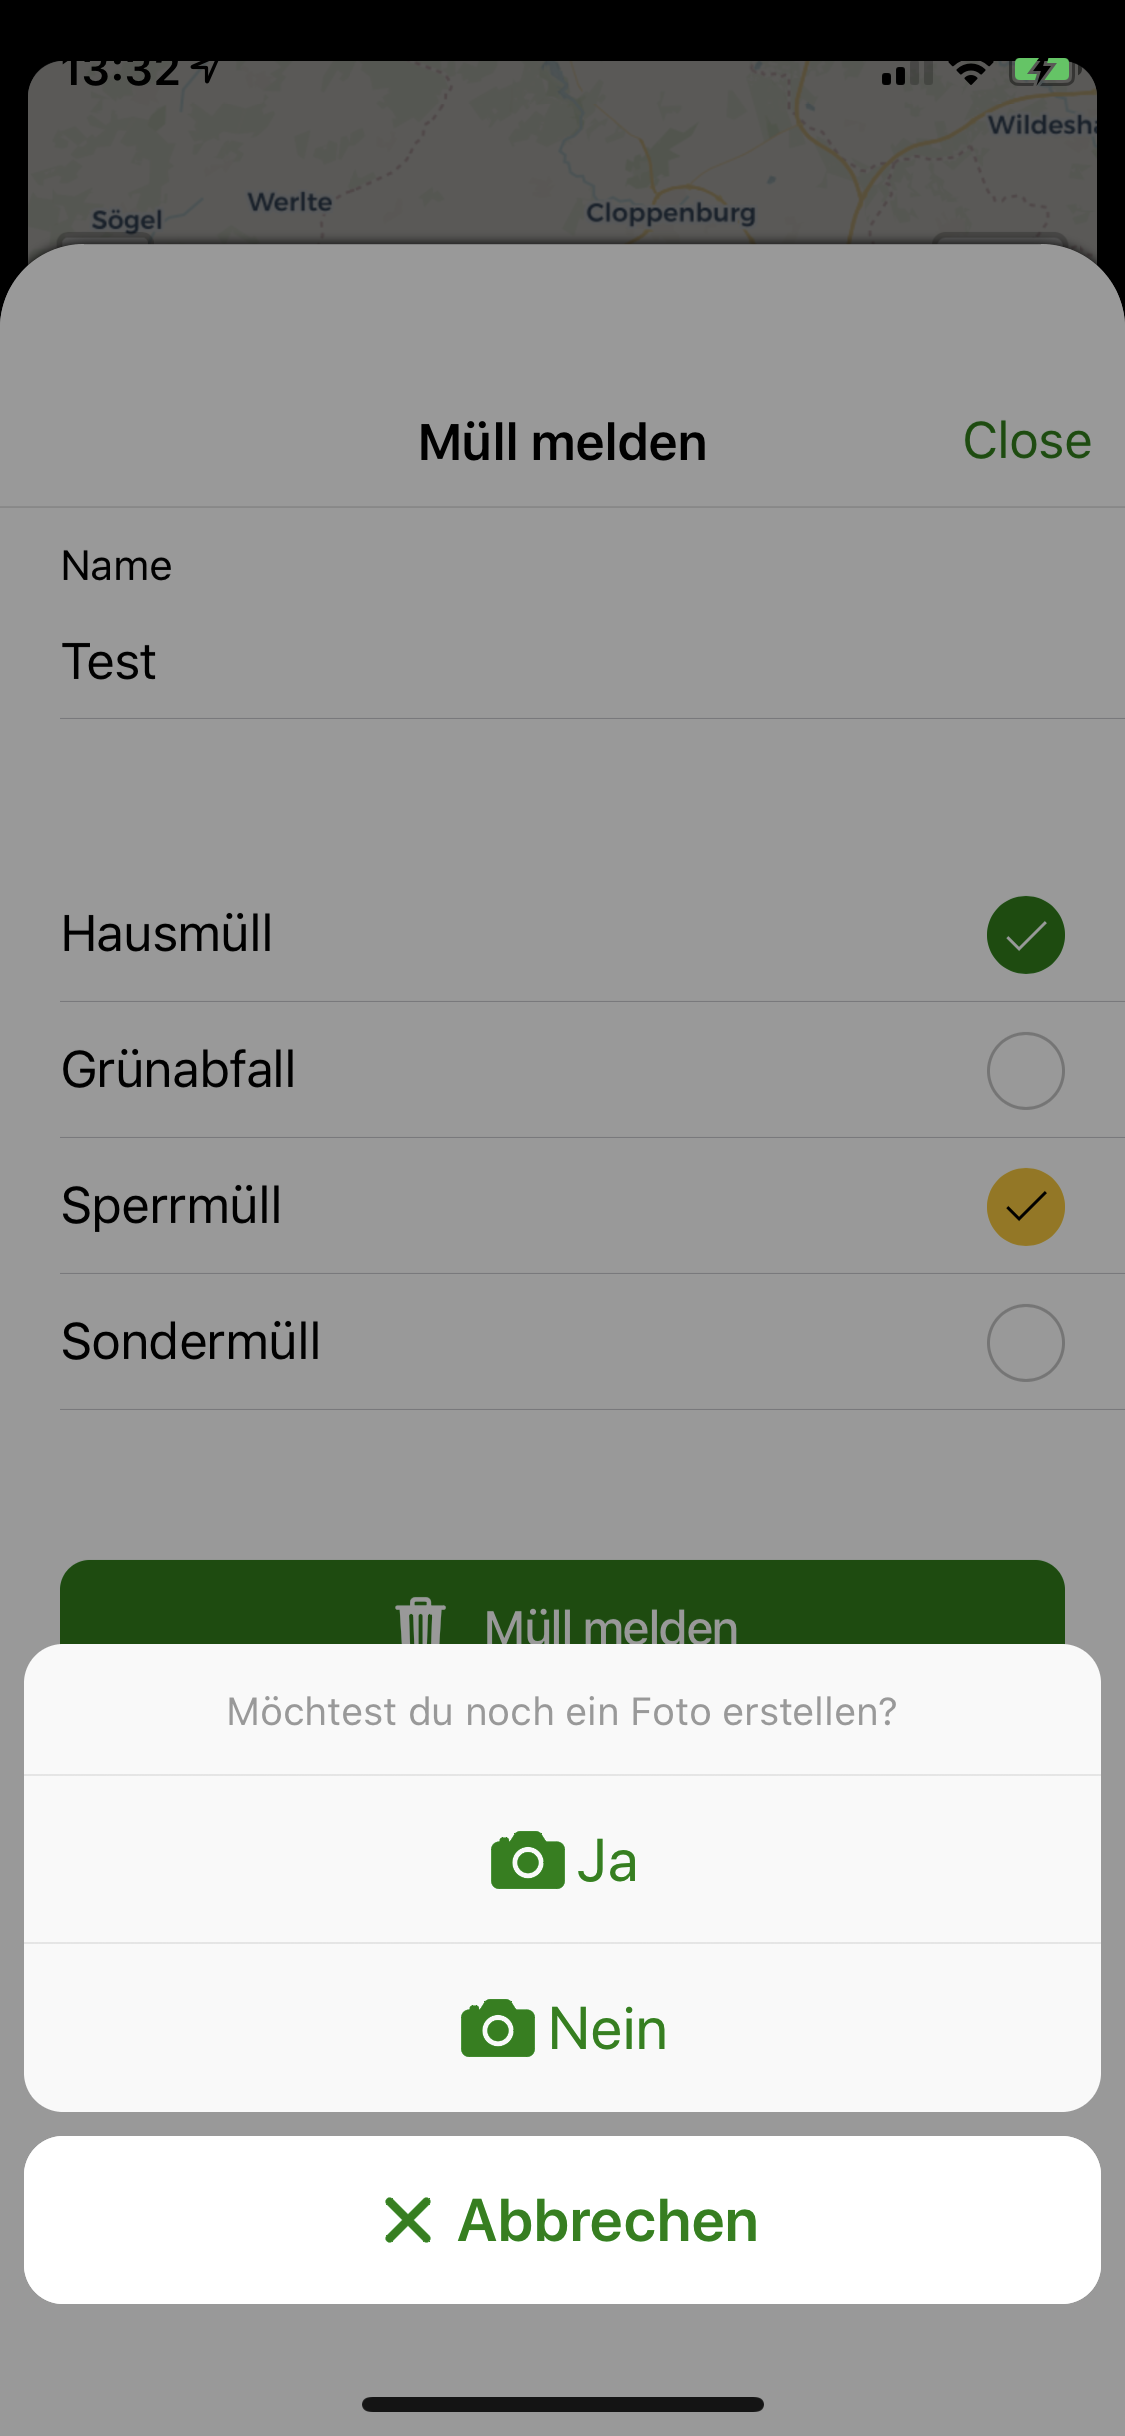
\includegraphics[width=0.2\textwidth]{img/app/report-photo.png}}\hfill%
		\subfigure[Fotoquelle wählen]{\centering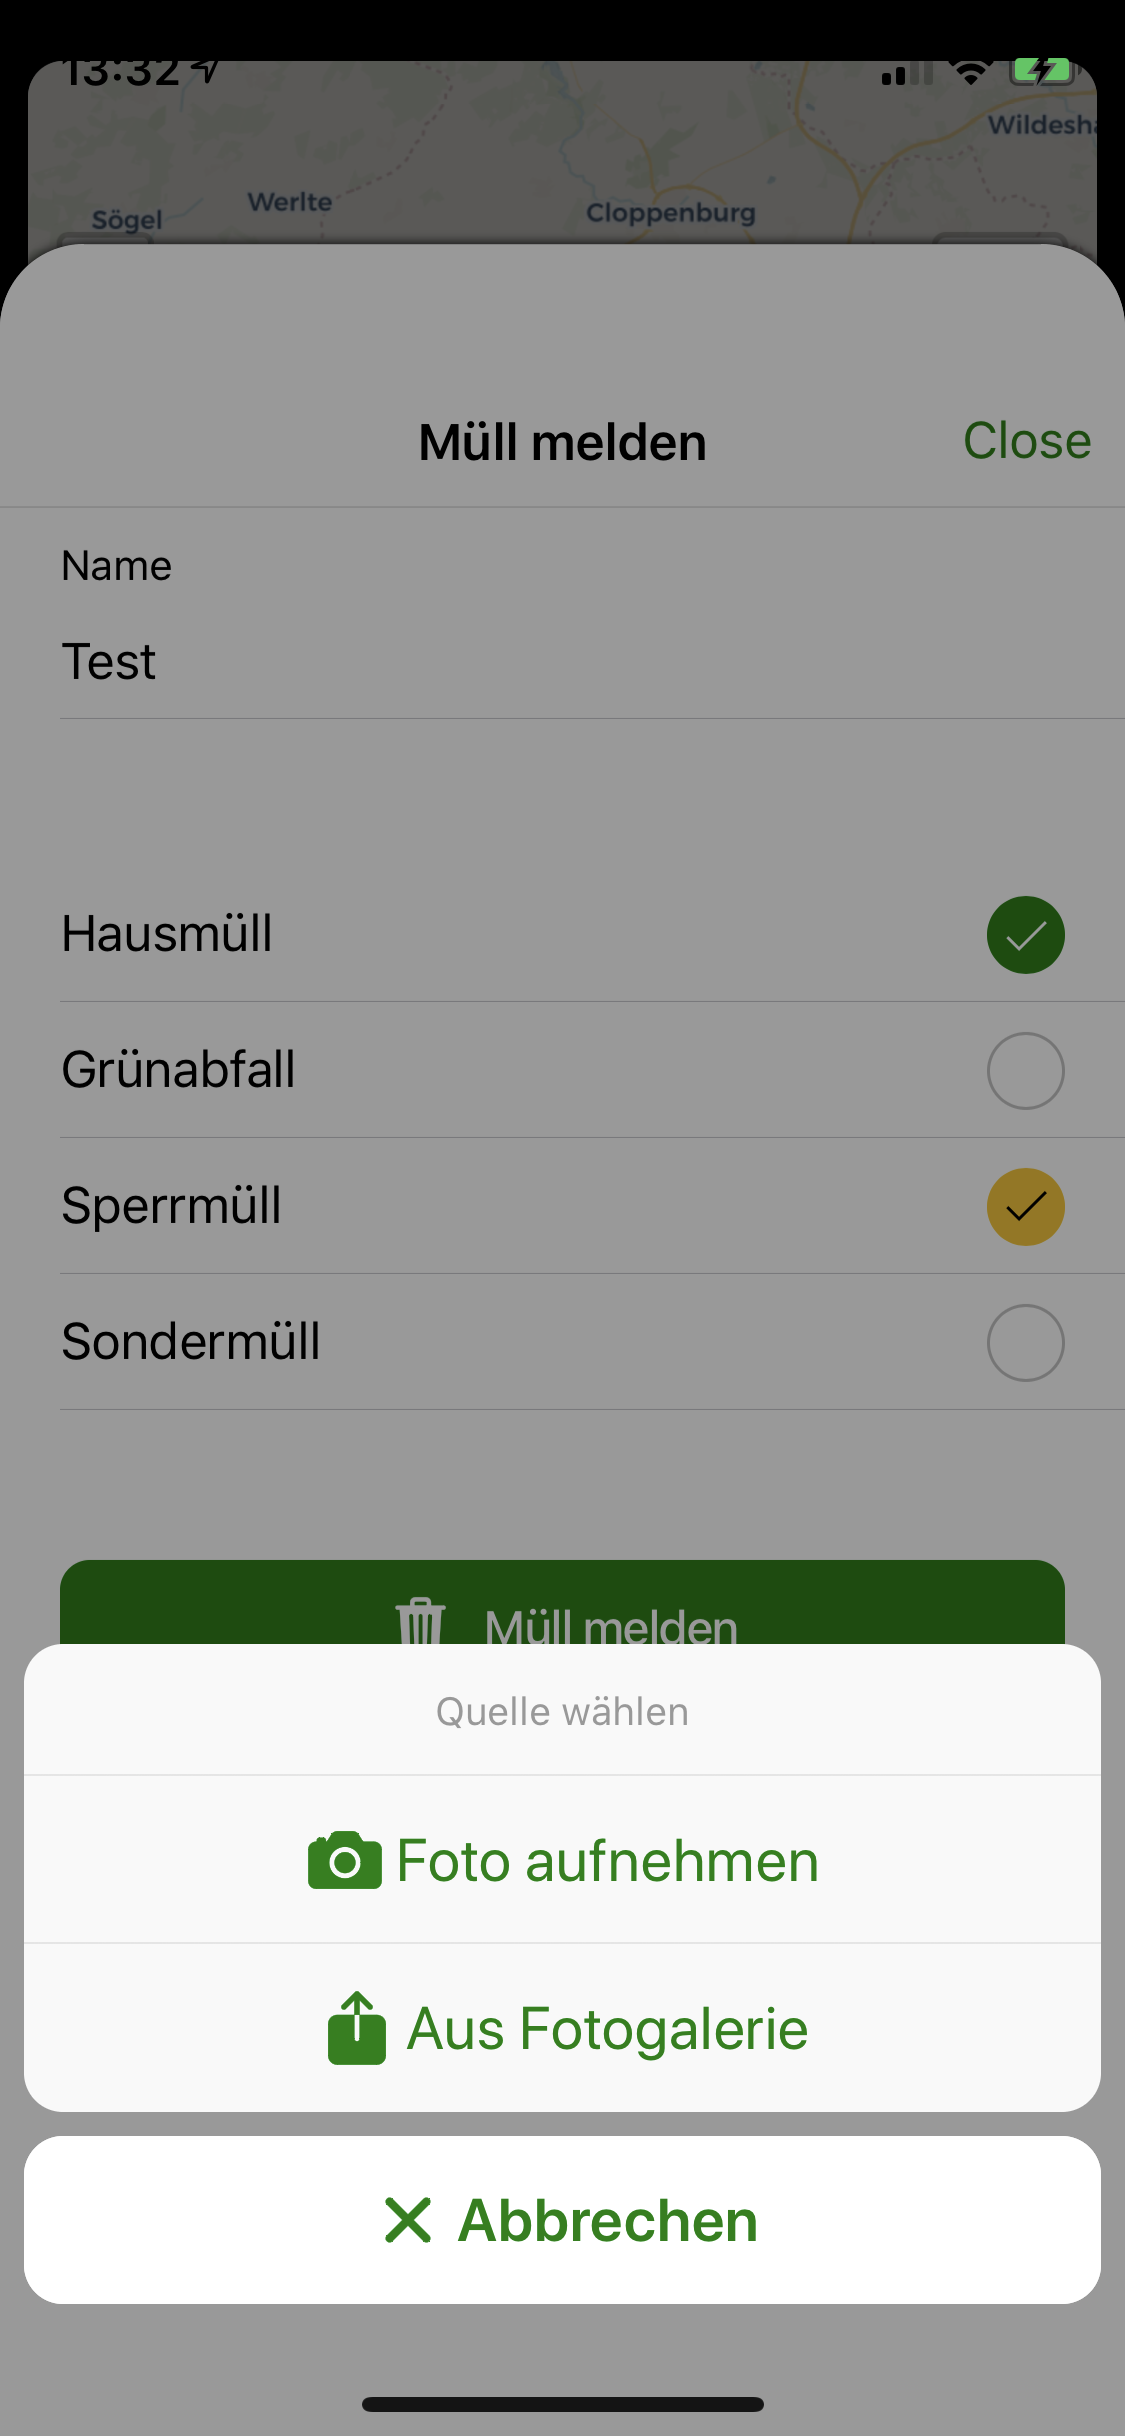
\includegraphics[width=0.2\textwidth]{img/app/report-photo-source.png}}\hfill%
		\subfigure[Bericht senden]{\centering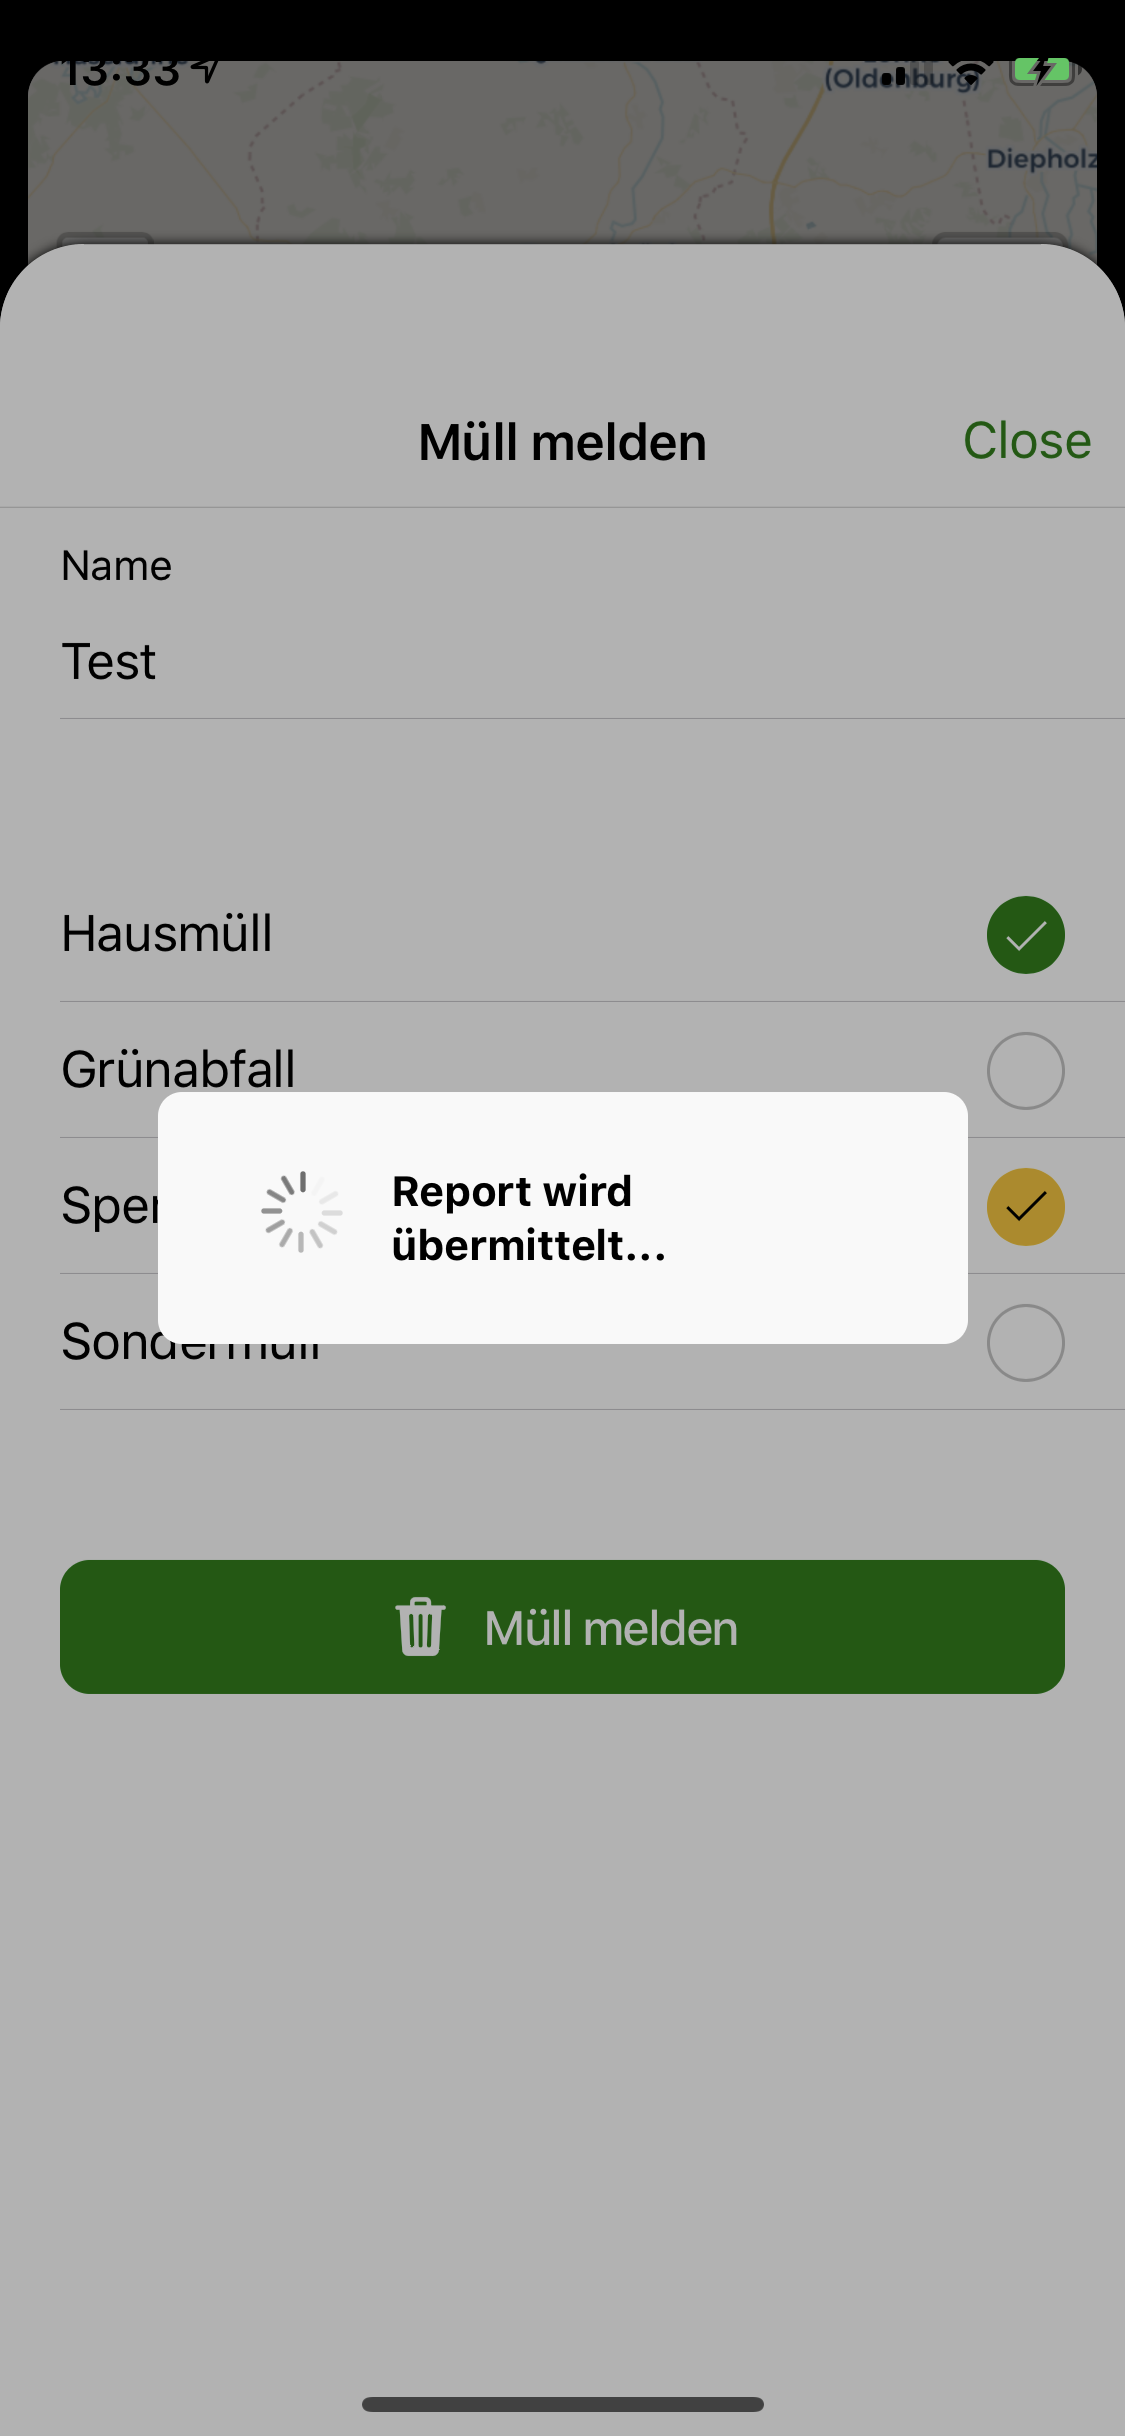
\includegraphics[width=0.2\textwidth]{img/app/report-send.png}}\hfill%
		\caption{Trash Report Add Page Modal}\label{fig:app-report}
	\end{figure}

	\paragraph{Filter}
	\textbf{}\\
	\textbf{}\\
	Um gewisse Filterfunktionalitäten bereitstellen zu können, wurde eine weitere Page-Komponente entwickelt, welche ebenfalls als \textit{Modal} realisiert wurde.
	Die Funktionsweise ist wie folgt:\\
	Über den \textit{Ionic Button} \textbf{Filter}, mittig am unteren Rand der Map-Page platziert, lässt sich einstellen, welche Meldungen von Müllablagerungen auf der Karte angezeigt werden sollen. Klickt man auf diesen Button, öffnet sich, wie auch bei der Müllmeldung, ein \textit{Ionic Modal}. In diesem lässt sich nach den folgenden Paramatern sortieren: \textit{Username}, \textit{Zeitraum}, \textit{Müllart} und einem \textit{Umgebungsradius}. Um einen Filter darzustellen, haben wir eine \textit{Typescript}-Klasse Filter angelegt, die die genannten Parameter abspeichert und mit \enquote{getter}- und \enquote{setter}-Methoden manipulierbar macht.
	Möchte der Nutzer beispielsweise nur Meldungen von der Nutzerin “Martha Musterfrau” angezeigt bekommen, die in einem Umkreis von 50 km um seinen aktuellen Standort gemeldet wurden, müssen zwei Einstellungen im Filter \textit{Modal} getroffen werden. Erstens wird der Nutzername in den \textit{Ionic} Input \enquote{Username} eingetippt und zweitens der \textit{Ionic} Slider auf den Wert 50, für den Radius in Kilometern, eingestellt.
	Da der Filter durch den \textit{Angular-Service \enquote{map.service}} bereitgestellt wird, können die Änderungen über die \textit{setFilters()}-Funktion direkt abgespeichert werden. Dann wird die \textit{applyFilters()}-Funktion mit \textit{true} als Übergabewert aufgerufen und der im \textit{mapService} hinterlegte Filter wird durch Serverabfragen angewendet, sodass nur noch die gewünschten Marker auf der Leaflet-Karte angezeigt werden.\\
	Um das Filter-Modal besser zu visualisieren, ist ein Screenshot hierzu in Abbildung \ref{fig:app-filter} zu sehen.
	\begin{figure}[!htbp]
		\centering
		\subfigure[Teil 1]{\centering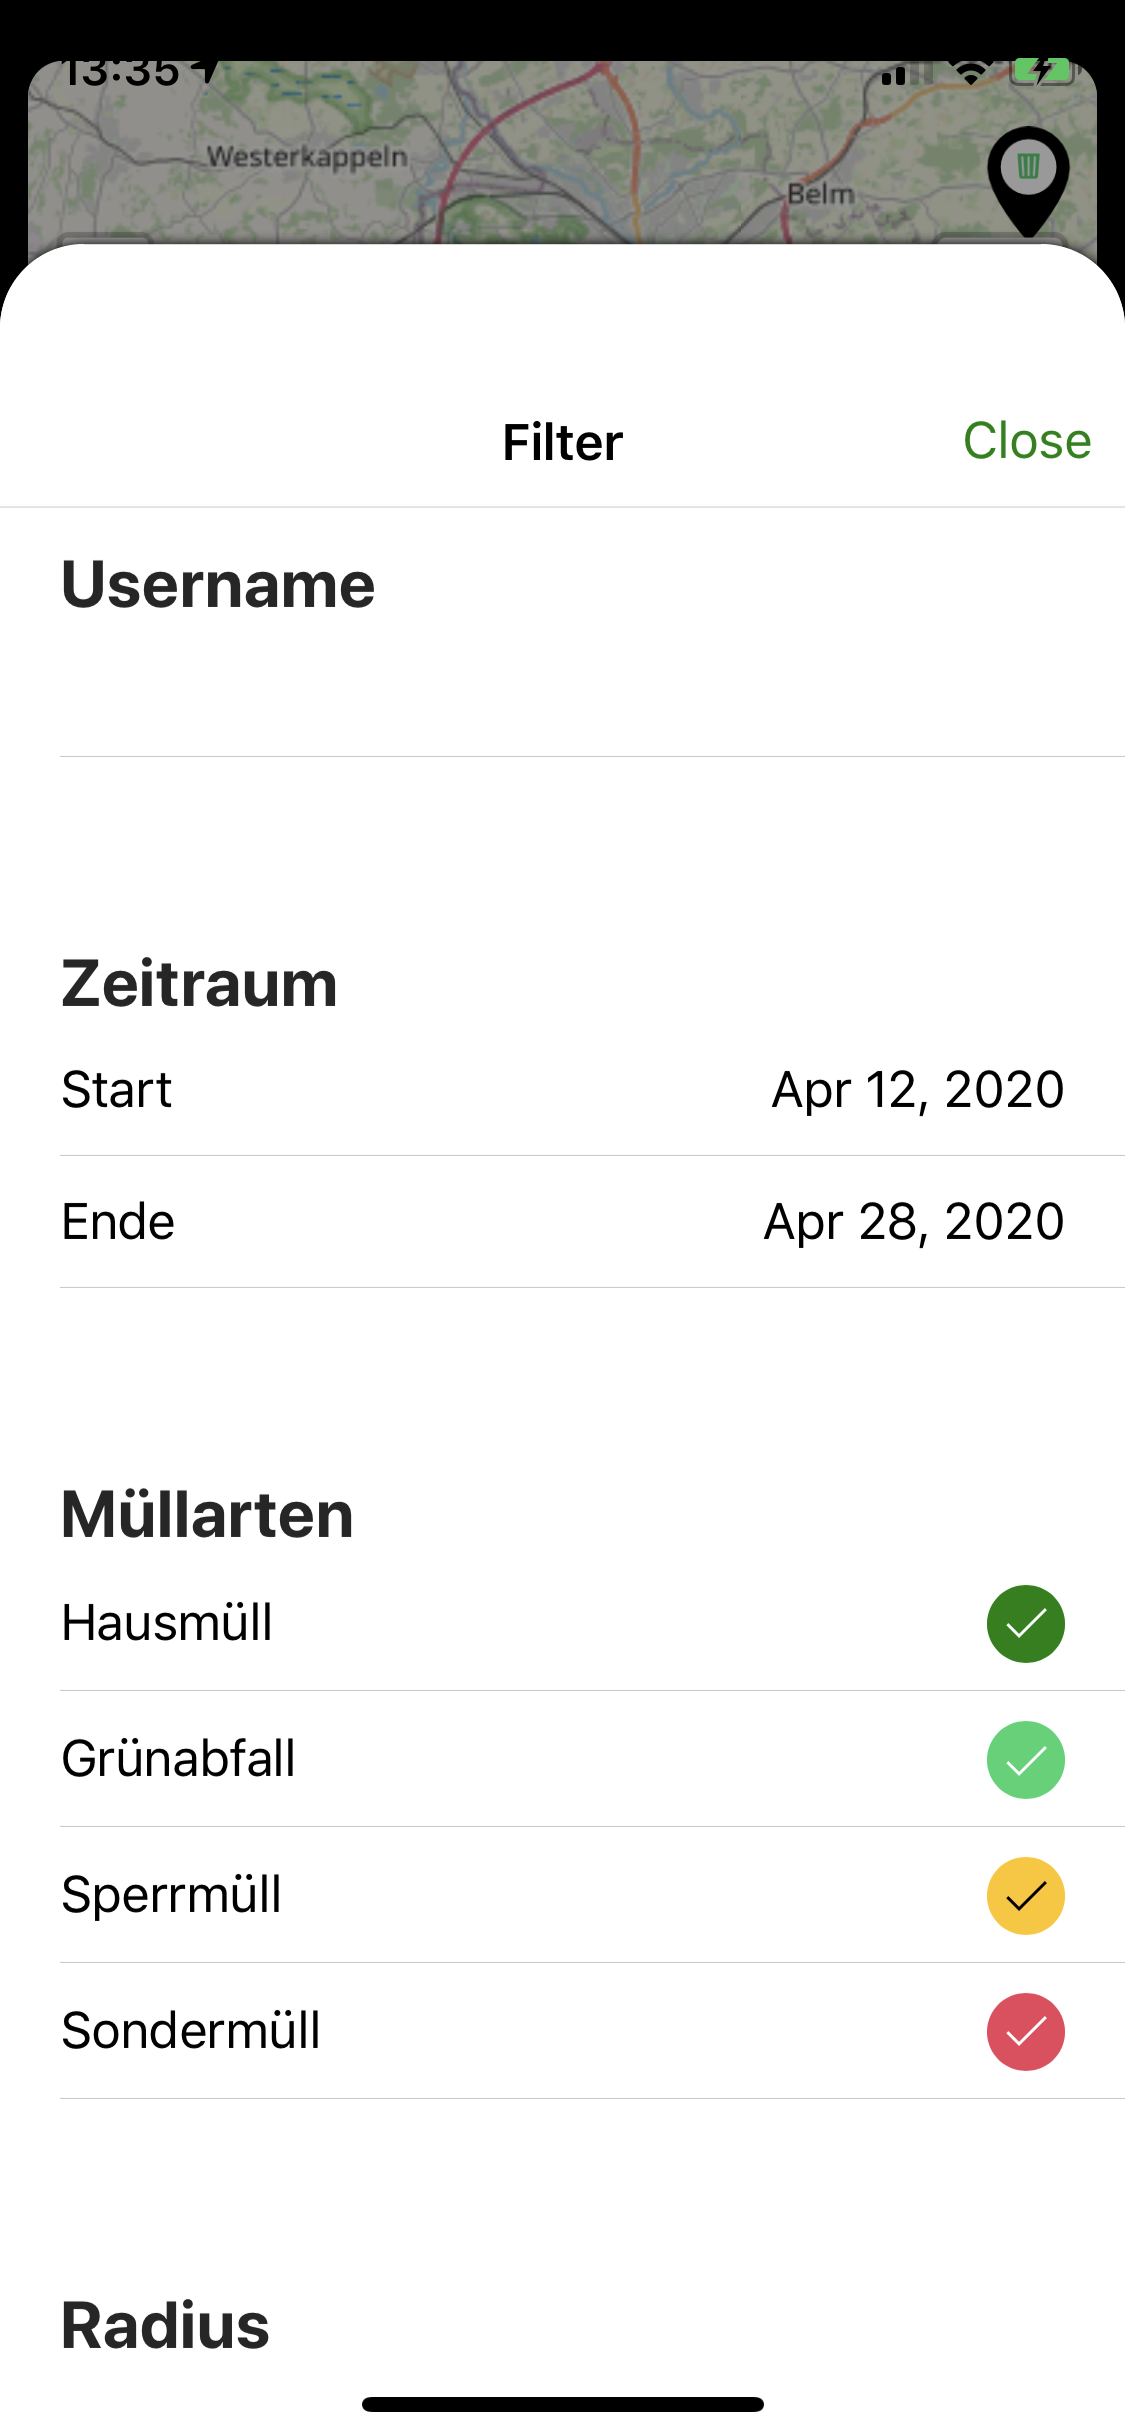
\includegraphics[width=0.3\textwidth]{img/app/filter-1.png}}\hfill%
		\subfigure[Teil 2]{\centering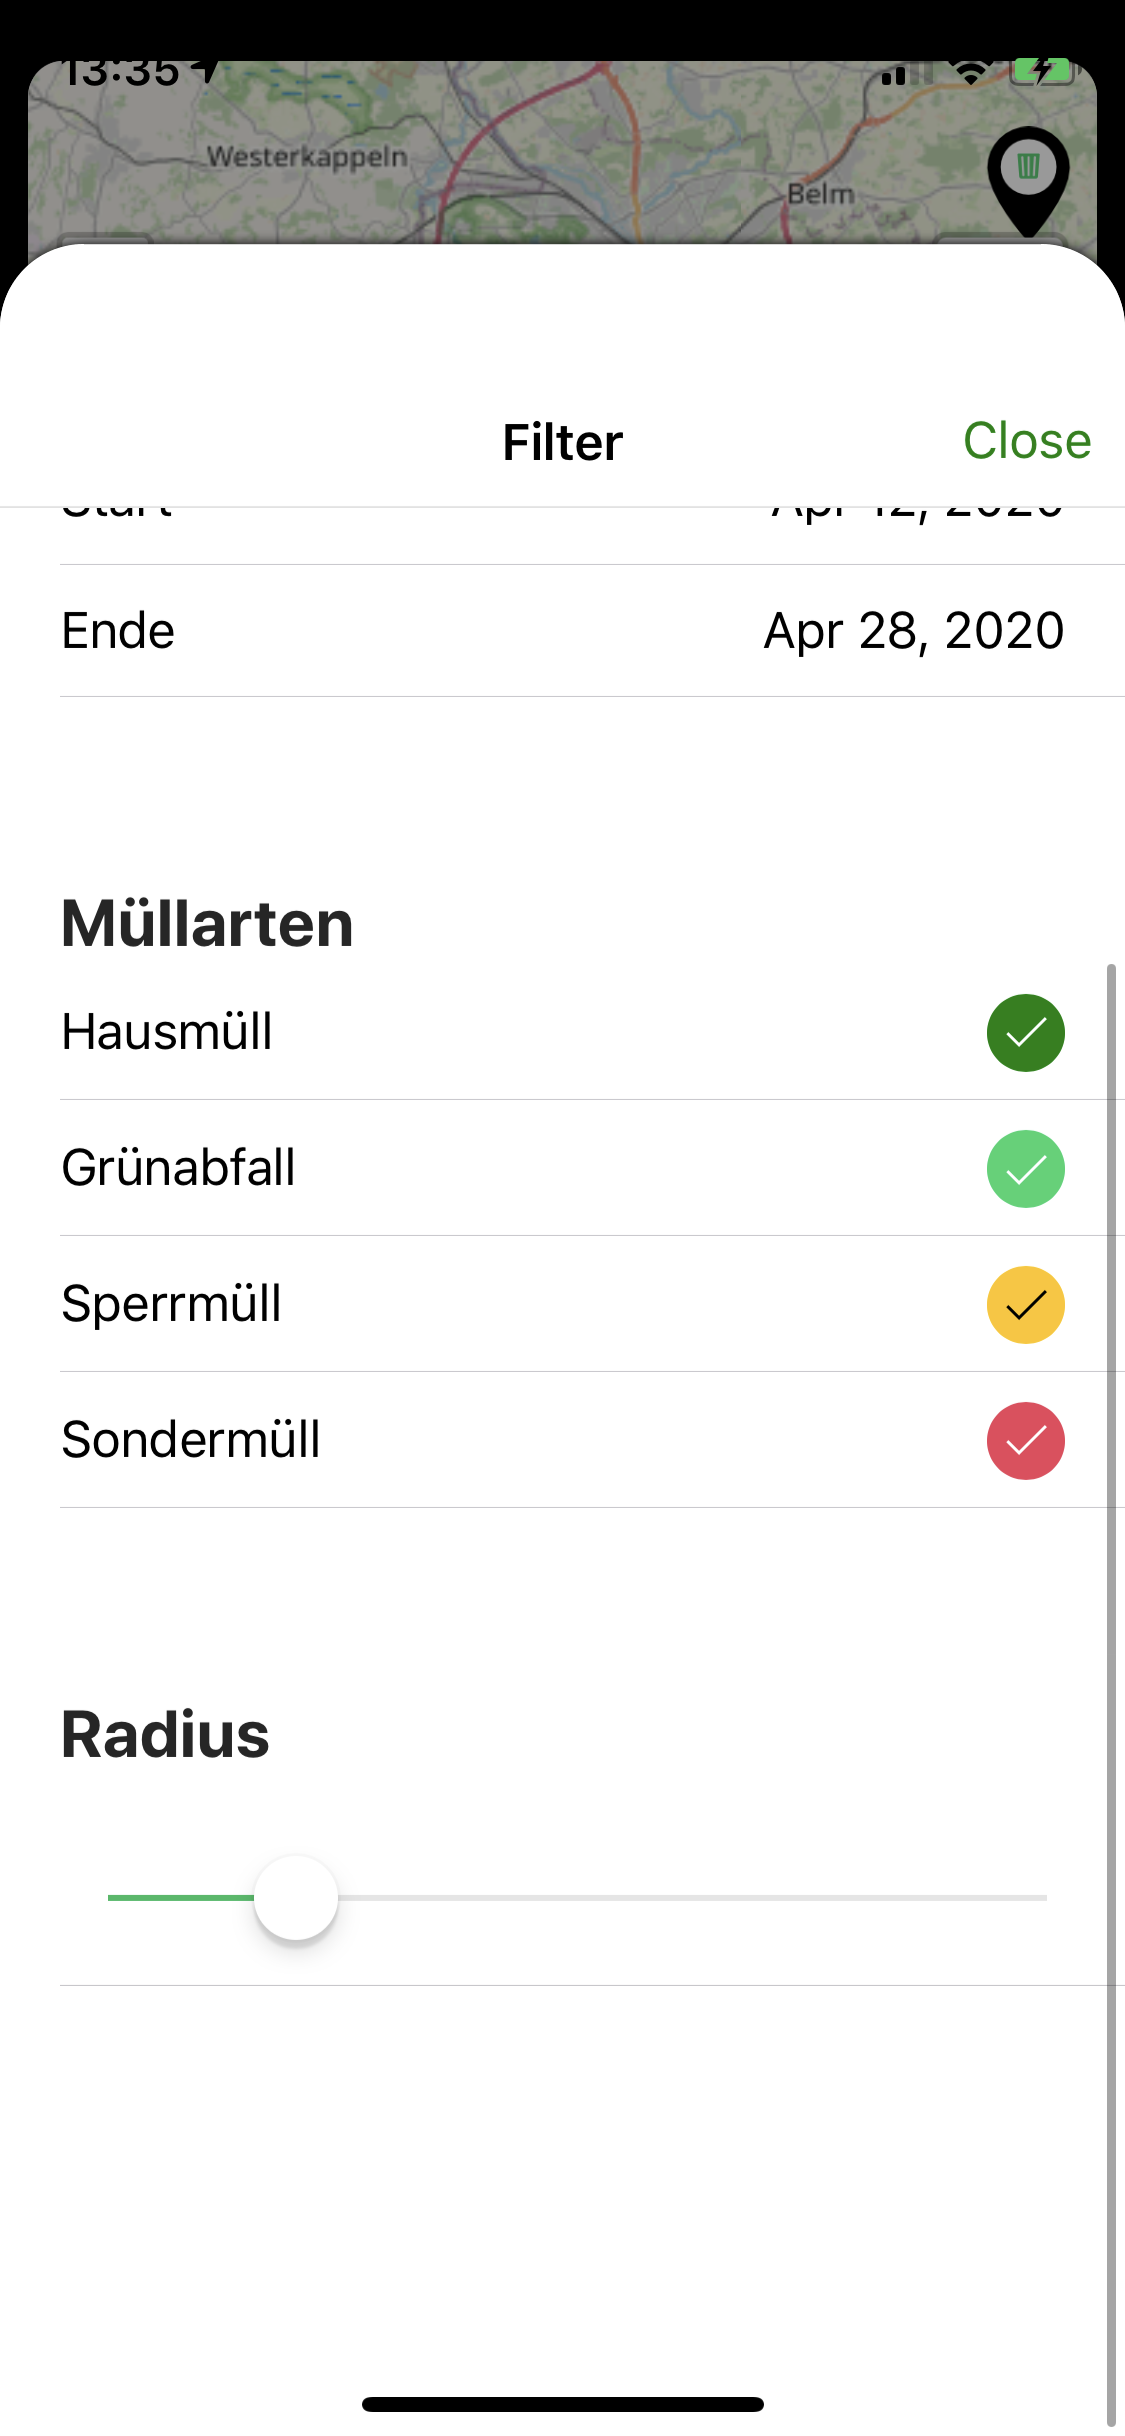
\includegraphics[width=0.3\textwidth]{img/app/filter-2.png}}\hfill%
		\caption{Filter Page Modal}\label{fig:app-filter}
	\end{figure}

	\subsubsection{Services}
	In diesem Abschnitt werden die entwickelten Angular-Services der App erläutert. Diese wurden genutzt, um zum Einen eine zentrale Stelle für die API-Kommunikation mit dem Server herzustellen und zum Anderen um die Datenstruktur für die Anwendung vorzuhalten (Caching).

	\paragraph{API}
	Der API-Service dient dazu eine zentrale HTTP-Kommunikation mit dem Server herzustellen. Dieser definiert die API-Calls zum Server und verarbeitet die Antwort des Servers.

	\paragraph{Map}
	Der Map-Service stellt einen zentralen Datenspeicher für die Anwendung dar. Hier werden Daten, wie die einzelnen Berichte zur Müllablagerung, vorgehalten (gecached), um diese nicht bei jeder Filteränderungen neu vom Server anzufragen.
	Zudem ist hierdurch einfach möglich, komponentenübergreifend, also sowohl in der Map-Komponente, als auch in den Modals auf die Datenstruktur zuzugreifen.
	
	\subsection{Backend / Server}
	\begin{itemize}
		\item In diesem Abschnitt wird erklärt wie der Server als Schnittstelle zwischen App und Datenbank fungiert. Die zwei Hauptfunktionen des Servers sind unter dem Endpoint \textit{/trash} mit HTTP-Get und POST erreichbar.
		\item Mit der GET-Methode werden die Anfragen der App nach Müllablagerungen bedient. Dort wird zuerst überprüft, ob die drei von der App zu sendeten Werte Latitude, Longitude und Radius wirklich gesendet wurden. Ist dies nicht der Fall wird der HTTP-Fehler 				400 (Bad Request) zurückgegeben. Danach wird geschaut, ob ein Start- und Enddatum vorhanden ist. Wenn keine Daten in der Filterfunktion der App angegeben wurden, werden die letzten 14 Tage als Anzeigezeitraum gewählt.
		\item Die zur Datenbankabfrage notwendigen Daten sind dann bereit, sodass folgendes Statement an die Datenbank geschickt werden kann:\textit{ “SELECT * FROM trash WHERE time BETWEEN startDate AND endDate ORDER BY id ASC”}. So bekommt man alle 				Müllablagerungsmeldungen zwischen Start- und Enddatum nach Meldezeitpunkt sortiert, da die \textit {id} als Primärschlüssel bei jeder Meldung hochgezählt wird.
			Die so erhaltenen Zeilen aus der Datenbank müssen noch auf den im Filter gewählten Radius ausgedünnt werden. Für die Berechnung wurde die Funktion \textit{getTrashDistance(center, marker)} geschrieben, um die Distanz auf der Erdkugel zu berechnen. 				Dabei enthält \textit{center} die Koordinaten des Nutzers, und \textit{marker} die der Müllmeldung. Die Koordinaten, der in dem Radius liegenden Meldungen, werden als Punkte im GeoJSON Format zurückgegeben. So können die Marker in der App an den 				passenden Punkten angezeigt werden.
		\item Die dritte Funktion des Servers ist es die vom Nutzer hochzuladenden Bilder anzunehmen. Zuerst wird überprüft, ob im empfangenen Body sich ein \textit{files}-Objekt befindet. Ist dies nicht der Fall wird der Statuscode 400 für Bad Request 							zurückgegeben. Das Foto wird mit dem eigenen md5-Hashwert als Dateinamen abgespeichert und an die App wird zusammen, mit Statuscode 200 der Dateipfad auf dem Server zurückgeschickt. Ansonsten kommt HTTP-Code 500 Internal Server Error, falls die 				Datei nicht abgespeichert werden kann.
	\end{itemize}

	\section{Zusammenfassung und Ausblick}
	Im Rahmen der Veranstaltung \enquote{Standortbasierte Dienste} im Wintersemester 2019/2020 wurde als Abschlussaufgabe ein prototypisches Müllmeldesystem zur Meldung illegaler Müllablagerungen entwickelt.
	Dieses besteht aus einem Frontend, realisiert als eine App mit dem \textit{Ionic Framework} in Kombination mit \textit{Apache Cordova}, sowie ein Backend, erstellt mit dem Framework \textit{Express.js}.\\
	Dieses konnte erfolgreich mit allen geforderten Funktionalitäten entwickelt werden. Zudem wurde die Möglichkeit eingebaut, die Berichte der Müllablagerungen zu filtern.
	Ebenso konnten verschiedene Ansätze hinsichtlich des Stylings eingebunden werden, welche die UX der Anwendung verbessern soll.\\
	Als Ausblick kann festgehalten werden, dass die App durch die prototypische Entwicklung noch weiter in Stabilität und Performanz verbessert werden kann.
	Zudem wurde die Möglichkeit gegeben, einzelne Berichte von Müllablagerungen in einer Art \enquote{Cache} abzulegen. Bei jeder Filteränderung wird jedoch eine komplette Liste weiterer Berichte angefordert und zurückgesendet, die dem Filter-Schema entsprechen und somit Duplikate enthalten kann, die zwar nicht in der App-Datenstruktur doppelt abgespeichert werden, jedoch die Datenmenge beim Anfragen vom Server reduziert werden könnte.
	Dies könnte realisiert werden, indem nur Berichte angefragt werden, die zum einem dem Filter-Schema entsprechen und zum Anderen noch nicht im Cache vorliegen. Dies wurde aus Gründen der Simplifizierung des Entwicklungsprozesses nicht implementiert.

	\printbibliography

	\textbf{}\\
	\section*{Abkürzungsverzeichnis}
	\begin{acronym}[API]
		\acro{API}{Application Programming Interface}
		\acro{HTTP}{Hypertext Transfer Protocol}
		\acro{REST}{REpresentational State Transfer}
		\acro{UI}{User Interface}
		\acro{UX}{User Experience}
	\end{acronym}
\end{document}